\documentclass{article}
\usepackage[utf8]{inputenc}
\usepackage{listings}

\title{EDA132 Project1 - Search}
\author{Lewis Belcher (900429-3552), Axel Larsson (920515-0395)}
\date{}

\usepackage{natbib}
\usepackage{graphicx}

\begin{document}

\maketitle

\section{Introduction}

\subsection{Outline}

In this project we use a simple MiniMax implementation to play the game of Reversi with Othello rules. Figure \ref{fig:othello-start} shows how the game starts with Othello rules. Player black moves first and the turns alternate between players while moves are available (play is given back to the opposition if no moves are available to the current player). The game is won by the player with the most tiles of their colour on the board when there are no more legal moves for either player.

\begin{figure}[h!]
\centering
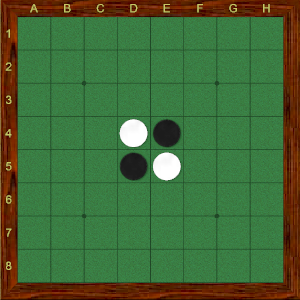
\includegraphics[scale=0.6]{othello-start.png}
\caption{Reversi with Othello rules starting position.}
\label{fig:othello-start}
\end{figure}

\subsection{Programming Language}

Python 3.4 was used as the programming language for this project.


\section{Implementation}

The board, game, human players and AI were implemented in an object oriented way with a lot of abstraction between classes. The board is first created along with two players which are then used to create a game instance. This game instance has a method \texttt{play} which is then used to play the game. 

The code is divided into two modules, both residing in the package \texttt{othello}; \texttt{game} and \texttt{players}. The \texttt{game} module has the implementations for the board representation, given by the class \texttt{Board} and the \texttt{Game} class. This is also where the main method resides to actually play the game. The \texttt{players} module has classes representing both the AI player, running the MiniMax algorithm, and the \texttt{Human} player which prompts the user for which move to make. There is another package containing tests for the respective modules, to be found in the directory \texttt{/h/d5/f/dat11al1/othello/tests}.

\subsection{Board}

The board was based largely on a \emph{numpy} array. Free spaces are represented by 0's and taken spaces are represented by the integer value of each player (each of which has their own implemented value, see the following subsection).

An ASCII representation of the board was implemented in this class where white is given by the ASCII letter \texttt{'O'} and black by \texttt{'*'}. An example of this is shown in Figure \ref{fig:ascii-board}. 

The file \texttt{/h/d5/f/dat11al1/othello/othello/game.py} contains the relevant code.

\begin{figure}[h!]
\centering
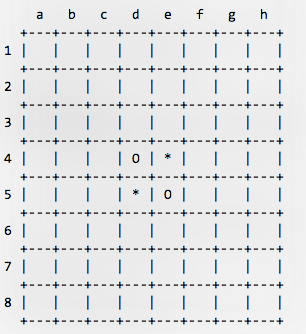
\includegraphics[scale=0.6]{ascii-board.png}
\caption{ASCII representation of the Board class.}
\label{fig:ascii-board}
\end{figure}

\subsection{Players}

The player colours \textit{white} and \textit{black} have integer representations of 1 and -1 respectively. In doing this it becomes trivial to sum up across all values on the board to determine who has the advantage. We make use of this implementation in the MiniMax algorithm in that the sum multiplied by the integer representation of the player is what we want to maximize (the converse for the minimizing step). The code for these classes can be found in \texttt{/h/d5/f/dat11al1/othello/othello/players.py}.

\subsection{Game}

The class \texttt{Game} is what runs and monitors the entire game. It is passed a board on which to play and two players. It contains various methods including checking for legal moves and determining which tiles must be flipped for a given move. The board is updated upon every move and the game keeps track of whose turn it is (including handing over play if there are no legal moves) and the outcome of the game. The code for this class can be found in \texttt{/h/d5/f/dat11al1/othello/othello/game.py}.


\subsection{MiniMax Algorithm}

The MiniMax algorithm used was adapted from the book \textit{Artificial Intelligence: A Modern Approach} \cite{Russell:2003:AIM:773294}. The implementation can be found under the class \texttt{MiniMaxAI} in \texttt{/h/d5/f/dat11al1/othello/othello/players.py}. The notion is to maximise the utility for the colour given at instantiation (as the first argument) under the assumption that the opposing player will move optimally. In our implementation we use a simple heuristic that a higher number of flipped tiles is favorable (this is a very naive heuristic but time did not permit us to implement more advanced techniques such as favorable positions or killer moves).


\subsection{Timing}

The time limit for the search was implemented in a very straightforward way:

\begin{enumerate}
    \item A time limit is set when creating an AI instance
    \item At the start of each search an attribute is set within the AI class which contains information of the current time
    \item After every step in the search \texttt{current time - time at start of the search} is checked to see if it exceeds the time limit set at instantiation, if it does then the search terminates
\end{enumerate}

\section{Usage}
The path to the program root is \texttt{/h/d5/f/dat11al1/othello}. While standing in that directory in the terminal, execute \texttt{python3 othello -h} to get a useful help text as such: 
\begin{lstlisting}
usage: othello [-h] [-v] [-t TIME]

Play othello vs an AI.

optional arguments:
  -h, --help            show this help message and exit
  -v, --visualise       visualise game board, default is
                        to output only AI moves
  -t TIME, --time TIME  time limit in seconds for each
                        ply, default is 10s
\end{lstlisting}

The \texttt{-t} option is used to indicate the amount of allotted time in seconds for the AI before making a decision on each ply. The \texttt{-v} flag can be used to get a nice ASCII visualisation of the game board. 

\subsection{Requirements}
The minimum requirements to execute the game is:
\begin{itemize}
    \item Python3
    \item numpy
\end{itemize}

If \texttt{virtualenv}, \texttt{setuptools} and \texttt{pip} is available on the system (which, unfortunately, they are not on the student computer system), these can be used to install the program in a virtual environment, but this is entirely optional.

\subsection{Playing}
While standing with the terminal in \texttt{/h/d5/f/dat11al1/othello}, type \texttt{python3 othello -v} to start the game with the ASCII visualisation. Add the \texttt{-t} option as explained in the previous section if a time limit other than 10 seconds is desired. If more machine-friendly output is required (i.e. no ASCII grid), the \texttt{-v} flag can be omitted.

While playing, the black player always starts and is assumed to be a human typing in the coordinates on the command line. The white player is the AI and will respond with its move.

\subsection{Testing}
While standing with the terminal in \texttt{/h/d5/f/dat11al1/othello/tests}, type \texttt{python3 game\_test.py} and \texttt{python3 players\_test.py} to unit test the modules \texttt{game} and \texttt{players} respectively.

\bibliographystyle{plain}
\bibliography{references}
\end{document}
